% Cheat Sheet
% Labels aren't necessary
%
% Chapter
%   \chapter{Chapter}\label{ch:chapter_1}
%
% Section
%   \section{Section}\label{sec:chapter_1/section_1}
%
% Subsection
%   \subsection{Subsection}\label{subsec:chapter_1/section_1/subsection_1}
%
% Unordered list
%   \begin{itemizePaper}
%       \item something;
%       \item something.
%   \end{itemizePaper}
%
% Numbered list
%   \begin{enumeratePaper}
%       \item Something.
%       \item Something.
%   \end{enumeratePaper}
<<<<<<< HEAD
\chapter{Моделирование температуры сольвуса никелевых жаропрочных сплавов с использованием нейронной сети}
=======
\chapter{Моделирование температуры сольвуса никелевых жаропрочных 
сплавов с использованием нейронной сети}
>>>>>>> master

\section{Теоретические основы}

\subsection{Никелевые жаропрочные сплавы и температура сольвуса}

<<<<<<< HEAD
Никелевые жаропрочные сплавы представляют собой сложнолегированные металлические материалы, предназначенные для работы при высоких температурах, механических нагрузках и агрессивных средах. Их высокая жаропрочность обусловлена многофазной структурой и наличием упрочняющих выделений, главным образом фаз $\gamma'$ и $\gamma''$.
Основой большинства никелевых суперсплавов является $\gamma$-матрица 
на основе никеля. В ней распределены частицы упрочняющей 
$\gamma'$-фазы. Также в зависимости от состава могут присутствовать карбиды, бориды и другие интерметаллидные соединения.

Одним из важнейших параметров, характеризующих фазовую стабильность никелевого жаропрочного сплава, является температура сольвуса $\gamma'$-фазы $T_{\mathrm{solvus}}$. Температура сольвуса соответствует температуре, выше которой упрочняющая фаза начинает растворяться в матрице. При превышении этой температуры структура сплава теряет устойчивость, что приводит к снижению прочностных характеристик.

Следовательно, прогнозирование температуры сольвуса по химическому составу является важной задачей при разработке новых жаропрочных сплавов и оптимизации уже существующих композиций.

\subsection{Влияние легирующих элементов}

Химический состав никелевых жаропрочных сплавов может включать большое количество элементов: Th, C, Cr, Co, Mo, W, Al, Ti, Nb, B, Fe, Y, Zr, Ta, Re, Ru, V, La, S, Si, Mn, P, Hf, Cu, Ge, Ga, Ni. Каждый из них выполняет определенную функцию.

Например, элементы Al, Ti, Ta и Nb участвуют в образовании упрочняющих интерметаллидных фаз. Cr и Al повышают стойкость к окислению и коррозии. Co, Mo, W, Re и Ta могут упрочнять твердый раствор. C, B, Zr и Hf влияют на границы зерен и образование карбидных фаз.

Влияние легирующих элементов является существенно нелинейным. Кроме того, один и тот же элемент может одновременно участвовать в нескольких физических механизмах. Поэтому построение простой аналитической зависимости между химическим составом и температурой сольвуса является затруднительным.
=======
Никелевые жаропрочные сплавы представляют собой сложнолегированные 
металлические материалы, предназначенные для работы при высоких 
температурах, механических нагрузках и агрессивных средах. Их высокая 
жаропрочность обусловлена многофазной структурой и наличием упрочняющих 
выделений, главным образом фаз $\gamma'$ и $\gamma''$.
Основой большинства никелевых суперсплавов является $\gamma$-матрица 
на основе никеля. В ней распределены частицы упрочняющей 
$\gamma'$-фазы. Также в зависимости от состава могут присутствовать 
карбиды, бориды и другие интерметаллидные соединения.

Одним из важнейших параметров, характеризующих фазовую стабильность 
никелевого жаропрочного сплава, является температура сольвуса 
$\gamma'$-фазы $T_{\mathrm{solvus}}$. Температура сольвуса соответствует 
температуре, выше которой упрочняющая фаза начинает растворяться в 
матрице. При превышении этой температуры структура сплава теряет 
устойчивость, что приводит к снижению прочностных характеристик.

Следовательно, прогнозирование температуры сольвуса по химическому 
составу является важной задачей при разработке новых жаропрочных 
сплавов и оптимизации уже существующих композиций.

\subsection{Влияние легирующих элементов}

Химический состав никелевых жаропрочных сплавов может включать 
большое количество элементов: Th, C, Cr, Co, Mo, W, Al, Ti, Nb, B, 
Fe, Y, Zr, Ta, Re, Ru, V, La, S, Si, Mn, P, Hf, Cu, Ge, Ga, Ni. 
Каждый из них выполняет определенную функцию.

Например, элементы Al, Ti, Ta и Nb участвуют в образовании 
упрочняющих интерметаллидных фаз. Cr и Al повышают стойкость к 
окислению и коррозии. Co, Mo, W, Re и Ta могут упрочнять твердый 
раствор. C, B, Zr и Hf влияют на границы зерен и образование карбидных фаз.

Влияние легирующих элементов является существенно нелинейным. Кроме 
того, один и тот же элемент может одновременно участвовать в нескольких 
физических механизмах. Поэтому построение простой аналитической 
зависимости между химическим составом и температурой сольвуса 
является затруднительным.
>>>>>>> master

\section{Описание модели}

\subsection{Нейронная сеть}

<<<<<<< HEAD
Для прогнозирования температуры сольвуса используется искусственная нейронная сеть прямого распространения. В общем виде модель можно записать следующим образом:
=======
Для прогнозирования температуры сольвуса используется искусственная 
нейронная сеть прямого распространения. В общем виде модель можно 
записать следующим образом:
>>>>>>> master

\begin{equation}
\hat{T}_{\mathrm{solvus}} =
f_{\theta}
\left(
x_1, x_2, \ldots, x_m
\right),
\end{equation}

<<<<<<< HEAD
где $\hat{T}_{\mathrm{solvus}}$ --- предсказанное значение температуры сольвуса, $x_i$ --- процентное сожержание легирующего элемента, $\theta$ --- обучаемые параметры модели.

Нейронная сеть выполняет роль нелинейного аппроксиматора, который устанавливает зависимость между химическим составом и температурой сольвуса. Преимущество такого подхода заключается в способности учитывать сложные нелинейные взаимодействия между элементами, которые трудно описать классическими аналитическими выражениями.

\subsection{Учет априорной физической информации}

Особенностью рассматриваемой модели является включение в архитектуру сети априорной информации о роли легирующих элементов. Элементы группируются по их влиянию на свойства сплава: твердорастворное упрочнение, образование карбидов, формирование $\gamma'$-фазы, повышение стойкости к окислению, стабилизация границ зерен и т.д.
=======
где $\hat{T}_{\mathrm{solvus}}$ --- предсказанное значение температуры 
сольвуса, $x_i$ --- процентное сожержание легирующего элемента, 
$\theta$ --- обучаемые параметры модели.

Нейронная сеть выполняет роль нелинейного аппроксиматора, который 
устанавливает зависимость между химическим составом и температурой 
сольвуса. Преимущество такого подхода заключается в способности 
учитывать сложные нелинейные взаимодействия между элементами, которые 
трудно описать классическими аналитическими выражениями.

\subsection{Учет априорной физической информации}

Особенностью рассматриваемой модели является включение в архитектуру 
сети априорной информации о роли легирующих элементов. Элементы 
группируются по их влиянию на свойства сплава: твердорастворное 
упрочнение, образование карбидов, формирование $\gamma'$-фазы, 
повышение стойкости к окислению, стабилизация границ зерен и т.д.
>>>>>>> master

Эта информация может быть представлена в виде матрицы связей:

\begin{equation}
R =
\left[
r_{gi}
\right],
\end{equation}

<<<<<<< HEAD
где $r_{gi}$ показывает, относится ли элемент $i$ к группе влияния $g$. Если элемент входит в соответствующую группу, то $r_{gi}=1$, иначе $r_{gi}=0$.
=======
где $r_{gi}$ показывает, относится ли элемент $i$ к группе влияния $g$. 
Если элемент входит в соответствующую группу, то $r_{gi}=1$, 
иначе $r_{gi}=0$.
>>>>>>> master

Для каждой группы можно сформировать обобщенный сигнал:

\begin{equation}
s_g =
\sum_{i=1}^{m}
r_{gi} x_i,
\end{equation}

где $s_g$ --- суммарный вклад элементов, относящихся к $g$-й группе.

<<<<<<< HEAD
Таким образом, нейронная сеть получает не только численные концентрации элементов, но и информацию об их физической роли в структуре сплава.
=======
Таким образом, нейронная сеть получает не только численные концентрации 
элементов, но и информацию об их физической роли в структуре сплава.
>>>>>>> master

\subsection{Дифференцирующий слой}

Дифференцирующий слой формирует два нелинейных преобразования входного
сигнала группы:
<<<<<<< HEAD
$$     \mathbf{p}_g =     \tanh \left(     W_g^{+}\mathbf{x}_g + \mathbf{b}_g^{+}     \right), $$
$$     \mathbf{n}_g =     \tanh \left(     W_g^{-}\mathbf{x}_g + \mathbf{b}_g^{-}     \right), $$
где $W_g^{+}$ и $W_g^{-}$ — обучаемые матрицы весов, а
$\mathbf{b}_g^{+}$ и $\mathbf{b}_g^{-}$ — векторы смещений. В данной
модели смещениям установлены значения
$$     \mathbf{b}_g^{+} = 0.5,     \qquad     \mathbf{b}_g^{-} = -0.5. $$

Дифференцированный сигнал определяется как разность двух нелинейных
преобразований:
$$     \mathbf{d}_g =     \mathbf{p}_g - \mathbf{n}_g. $$
=======
$$\mathbf{p}_g =\tanh \left(W_g^{+}\mathbf{x}_g + \mathbf{b}_g^{+}\right),$$
$$\mathbf{n}_g =\tanh \left(W_g^{-}\mathbf{x}_g + \mathbf{b}_g^{-}\right),$$
где $W_g^{+}$ и $W_g^{-}$ — обучаемые матрицы весов, а
$\mathbf{b}_g^{+}$ и $\mathbf{b}_g^{-}$ — векторы смещений. В данной
модели смещениям установлены значения
$$\mathbf{b}_g^{+} = 0.5,\qquad\mathbf{b}_g^{-} = -0.5.$$

Дифференцированный сигнал определяется как разность двух нелинейных
преобразований:
$$\mathbf{d}_g =\mathbf{p}_g - \mathbf{n}_g.$$
>>>>>>> master
Такое представление позволяет сети учитывать не только суммарное
содержание элементов в группе, но и различия в характере их влияния на
целевое свойство.

Выход $g$-й ветви дифференцирующего слоя записывается в виде
<<<<<<< HEAD
$$     \mathbf{h}_g =     \left[     s_g,\;     \mathbf{p}_g,\;     \mathbf{n}_g,\;     \mathbf{d}_g     \right]. $$
После обработки всех групп выходные векторы объединяются:
$$     \mathbf{h} =     \left[     \mathbf{h}_1,\mathbf{h}_2,\ldots,\mathbf{h}_G     \right], $$
=======
$$\mathbf{h}_g =\left[s_g,\;\mathbf{p}_g,\;\mathbf{n}_g,\;\mathbf{d}_g\right].$$
После обработки всех групп выходные векторы объединяются:
$$\mathbf{h} =\left[\mathbf{h}_1,\mathbf{h}_2,\ldots,\mathbf{h}_G\right],$$
>>>>>>> master
где $G$ — число групп легирующих элементов.

Итоговый вход последующей полносвязной части сети формируется путем
объединения исходного вектора состава и группового дифференцированного
сигнала:
<<<<<<< HEAD
$$     \mathbf{z} =     \left[     \mathbf{x},\mathbf{h}     \right]. $$
Затем вектор $\mathbf{z}$ поступает на полносвязную нейронную сеть:
$$     \hat{y}     =     f_{\theta}(\mathbf{z}), $$
=======
$$\mathbf{z} = \left[\mathbf{x},\mathbf{h}\right].$$
Затем вектор $\mathbf{z}$ поступает на полносвязную нейронную сеть:
$$\hat{y}=f_{\theta}(\mathbf{z}),$$
>>>>>>> master
где $\hat{y}$ — прогнозируемое значение температуры сольвуса, а
$f_{\theta}$ — обучаемая нелинейная функция, реализуемая скрытыми
слоями нейронной сети.

Таким образом, дифференцирующий слой выполняет две функции. Во-первых,
он внедряет в архитектуру сети априорную информацию о физической роли
легирующих элементов. Во-вторых, он формирует дополнительные нелинейные
признаки, описывающие групповой и дифференцированный вклад элементов в
прогнозируемое свойство.

\section{Реализация модели}

\subsection{Общая схема вычислительного эксперимента}

Реализация модели включает следующие этапы:

\begin{enumeratePaper}
<<<<<<< HEAD
    \item формирование матрицы связей, описывающей физическую роль легирующих элементов;
=======
    \item формирование матрицы связей, описывающей физическую роль 
    легирующих элементов;
>>>>>>> master
    \item построение глубокой нейронной сети с дифференциальным слоем;
    \item обучение модели на подготовленных данных;
    \item оценка точности прогноза по выбранным метрикам.
\end{enumeratePaper}

\subsection{Метрики качества}

<<<<<<< HEAD
Для оценки качества прогноза могут использоваться относительная средняя абсолютная ошибка и относительная среднеквадратичная ошибка.
=======
Для оценки качества прогноза могут использоваться относительная средняя 
абсолютная ошибка и относительная среднеквадратичная ошибка.
>>>>>>> master

Относительная средняя абсолютная ошибка определяется выражением:

\begin{equation}
RMAE =
\frac{1}{n}
\sum_{i=1}^{n}
\left|
\frac{T_i - \hat{T}_i}{T_i}
\right| \cdot 100\%,
\end{equation}

где $T_i$ --- экспериментальное значение температуры сольвуса, $\hat{T}_i$ --- предсказанное значение, $n$ --- количество объектов в выборке.

Относительная среднеквадратичная ошибка определяется как:

\begin{equation}
RRMSE =
\sqrt{
\frac{1}{n}
\sum_{i=1}^{n}
\left(
\frac{T_i - \hat{T}_i}{T_i}
\right)^2
}.
\end{equation}

\section{Результаты моделирования}

В результате применения нейронной сети была получена модель, способная 
прогнозировать температуру сольвуса никелевых жаропрочных сплавов по 
их химическому составу. Использование априорной информации о роли элементов 
позволило повысить физическую обоснованность входных данных.

По данным воспроизводимой статьи, модель показала достаточно высокую 
точность: относительная средняя абсолютная ошибка составила около 
$RMAE = 5.89\%$, а относительная среднеквадратичная ошибка --- около $RRMSE = 0.09$.

\subsection{Точечные результаты на тестовой выборке}
На тестовой выборке были получены предсказания $\hat{y}$ и вычислены ошибки. 
Для иллюстрации качества работы модели в таблице приведены 5 случаев с 
наибольшими значениями ошибки на тесте.

\begin{table}[h!]
\centering
\begin{tabular}{|r|r|r|r|}
\hline
$y_{\mathrm{true}}$ & $y_{\mathrm{pred}}$ & $|e|$ & $rel\_error(\%)$ \\
\hline
% 5 строк
<<<<<<< HEAD
... & ... & ... & ... \\ \hline
... & ... & ... & ... \\ \hline
... & ... & ... & ... \\ \hline
... & ... & ... & ... \\ \hline
... & ... & ... & ... \\ \hline
\end{tabular}
\end{table}

\subsection{Оценка качества модели по кросс-валидации}
Для проверки устойчивости обучения использовалась кросс-валидация: модель переобучалась на каждом фолде и вычислялись метрики.
=======
773.15 & 1191.20 & 418.05 & 54.07 \\ \hline
973.15 & 1285.83 & 312.68 & 32.13 \\ \hline
1023.15 & 1224.65 & 201.50 & 19.69 \\ \hline
1373.15 & 1154.06 & 219.08 & 15.95 \\ \hline
1143.15 & 967.36 & 175.78 & 15.37 \\ \hline
\end{tabular}
\captionsetup{justification=centering}
\caption{Пять худших предсказаний на тестовой выборке}
\label{tab:worst_predictions_test}
\end{table}

\subsection{Оценка качества модели по кросс-валидации}
Для проверки устойчивости обучения использовалась кросс-валидация: 
модель переобучалась на каждом фолде и вычислялись метрики.
>>>>>>> master
Итоговые значения представлены медианой и дисперсией по фолдам.

\begin{table}[h!]
\centering
<<<<<<< HEAD
\caption{Сводные результаты кросс-валидации (медиана и дисперсия)}
\label{tab:cv_summary}
=======
>>>>>>> master
\begin{tabular}{|l|c|c|}
\hline
Метрика & Медиана & Дисперсия \\
\hline
<<<<<<< HEAD
RRMAE (\%) & ... & ... \\
RRMSE & ... & ... \\
\hline
\end{tabular}
\end{table}

\subsection{Неопределённость метрик по методу бутстрэпа}
Для дополнительно оценки устойчивости метрик вычислялись распределения RRMAE и RRMSE с помощью бутстрэпа.
Квантили 2.5\% и 97.5\% соответствуют приближённому доверительному интервалу, а вертикальная линия (медиана) показывает центральную тенденцию.
Рисунки~\ref{fig:bootstrap_rrmae}--\ref{fig:bootstrap_rrmse} иллюстрируют полученные распределения.
=======
RRMAE (\%) & 4.36 & 0.79 \\
RRMSE & 0.08 & 0.0001 \\
\hline
\end{tabular}
\captionsetup{justification=centering}
\caption{Сводные результаты кросс-валидации}
\label{tab:cv_summary}
\end{table}

\subsection{Неопределённость метрик по методу бутстрэпа}
Для дополнительно оценки устойчивости метрик вычислялись распределения 
RRMAE и RRMSE с помощью бутстрэпа.
Квантили 2.5\% и 97.5\% соответствуют приближённому доверительному 
интервалу, а вертикальная линия (медиана) показывает центральную 
тенденцию.
Рисунки~\ref{fig:bootstrap_rrmae}--\ref{fig:bootstrap_rrmse} иллюстрируют 
полученные распределения.
>>>>>>> master

\begin{figure}[h!]
\centering
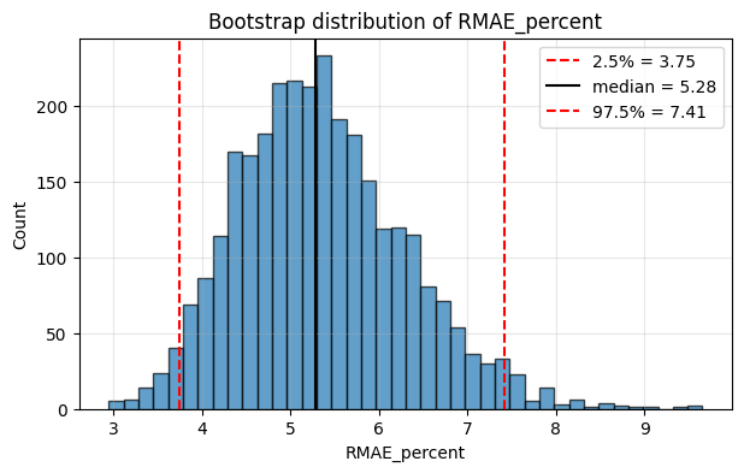
\includegraphics[width=0.75\textwidth]{../images/bootstrap_RRMAE.png}
\caption{Распределение RRMAE (\%) по бутстрэп-выборкам}
\label{fig:bootstrap_rrmae}
\end{figure}

\begin{figure}[h!]
\centering
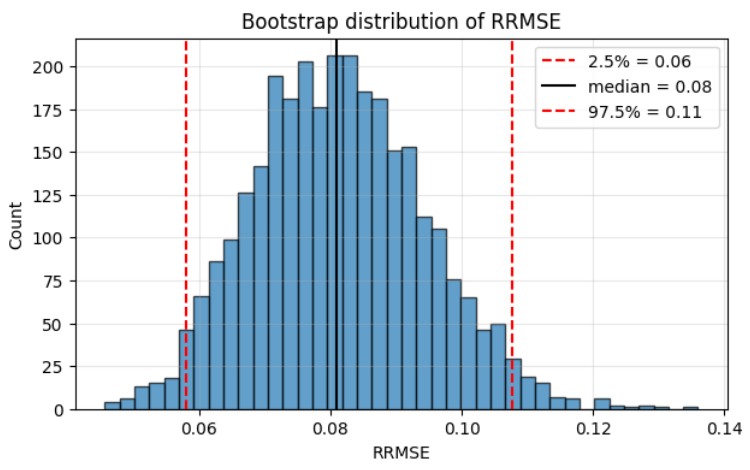
\includegraphics[width=0.75\textwidth]{../images/bootstrap_RRMSE.png}
\caption{Распределение RRMSE по бутстрэп-выборкам}
\label{fig:bootstrap_rrmse}
\end{figure}

<<<<<<< HEAD

\section{Выводы по главе}

Полученные результаты показывают, что нейронная сеть с дифференциальным слоем может быть использована для прогнозирования температуры сольвуса сложнолегированных никелевых суперсплавов. Такой подход особенно эффективен в условиях, когда аналитическое описание зависимости между составом и свойствами затруднено из-за высокой нелинейности и многокомпонентности системы.

В данной главе рассмотрен подход к моделированию температуры сольвуса никелевых жаропрочных сплавов с использованием глубокой нейронной сети. Основными особенностями модели являются:
=======
Итак, таблица~\ref{tab:worst_predictions_test} показывает поведение модели 
на тесте в наиболее проблемных случаях, кросс-валидация (табл.~\ref{tab:cv_summary}) 
оценивает устойчивость качества при повторном обучении на различных фолдах, 
а бутстрэп (рис.~\ref{fig:bootstrap_rrmae}--\ref{fig:bootstrap_rrmse}) предоставляет 
распределения метрик и их доверительные интервалы.

\newpage

\section{Выводы по главе}

Полученные результаты показывают, что нейронная сеть с дифференциальным 
слоем может быть использована для прогнозирования температуры сольвуса 
сложнолегированных никелевых суперсплавов. Такой подход особенно 
эффективен в условиях, когда аналитическое описание зависимости между 
составом и свойствами затруднено из-за высокой нелинейности и 
многокомпонентности системы.
 
Основными особенностями модели являются:
>>>>>>> master

\begin{itemizePaper}
    \item учет физической роли легирующих элементов;
    \item применение дифференциального слоя для анализа чувствительности модели.
\end{itemizePaper}

<<<<<<< HEAD
Итак, таблица~\ref{tab:worst_predictions_test} показывает поведение модели на тесте в наиболее проблемных случаях, 
кросс-валидация (табл.~\ref{tab:cv_summary}) оценивает устойчивость качества при повторном обучении на различных фолдах, 
а бутстрэп (рис.~\ref{fig:bootstrap_rrmae}--\ref{fig:bootstrap_rrmse}) предоставляет распределения метрик и их доверительные интервалы.


\chapter{Прогнозирование жаропрочности никелевых суперсплавов с использованием BRANN и параметра Ларсона--Миллера}
=======

\chapter{Прогнозирование жаропрочности никелевых суперсплавов с 
использованием BRANN и параметра Ларсона--Миллера}
>>>>>>> master

\section{Теоретические основы}

\subsection{Жаропрочность никелевых суперсплавов}

<<<<<<< HEAD
Жаропрочность является одной из ключевых характеристик никелевых суперсплавов. Она определяет способность материала сохранять прочность при длительном воздействии высокой температуры и механической нагрузки.

В условиях высокотемпературной эксплуатации структура суперсплава постепенно деградирует. Происходит укрупнение упрочняющих фаз, изменение морфологии выделений, перераспределение легирующих элементов и накопление повреждений. В результате предел прочности $\sigma$ снижается.

Для описания изменения прочности при различных температурах и временах выдержки удобно использовать обобщенные температурно-временные параметры. Одним из наиболее распространенных является параметр Ларсона--Миллера.

\subsection{Параметр Ларсона--Миллера}

Параметр Ларсона--Миллера объединяет температуру и время выдержки в одну величину:
=======
Жаропрочность является одной из ключевых характеристик никелевых 
суперсплавов. Она определяет способность материала сохранять прочность 
при длительном воздействии высокой температуры и механической нагрузки.

В условиях высокотемпературной эксплуатации структура суперсплава 
постепенно деградирует. Происходит укрупнение упрочняющих фаз, 
изменение морфологии выделений, перераспределение легирующих элементов и 
накопление повреждений. В результате предел прочности $\sigma$ снижается.

Для описания изменения прочности при различных температурах и временах 
выдержки удобно использовать обобщенные температурно-временные параметры. 
Одним из наиболее распространенных является параметр Ларсона--Миллера.

\subsection{Параметр Ларсона--Миллера}

Параметр Ларсона--Миллера объединяет температуру и время выдержки в 
одну величину:
>>>>>>> master

\begin{equation}
P_{LM} =
T
\left(
20 + \log_{10}\tau
\right),
\end{equation}

<<<<<<< HEAD
где $T$ --- температура испытания, $\tau$ --- время выдержки или длительность испытания.
=======
где $T$ --- температура испытания, $\tau$ --- время выдержки или 
длительность испытания.
>>>>>>> master

В рассматриваемой работе используется нормированная форма параметра:

\begin{equation}
P_{LM}^{*} =
T
\left(
20 + \log_{10}\tau
\right)
\cdot 10^{-5}.
\end{equation}

<<<<<<< HEAD
Нормировка необходима для того, чтобы значения параметра Ларсона--Миллера были сопоставимы по порядку величины с концентрациями легирующих элементов, используемыми как входные признаки нейронной сети.

Параметр $P_{LM}^{*}$ отражает степень температурно-временного воздействия на материал. При увеличении этого параметра прочность сплава, как правило, снижается вследствие термической деградации структуры.
=======
Нормировка необходима для того, чтобы значения параметра Ларсона--Миллера 
были сопоставимы по порядку величины с концентрациями легирующих элементов, 
используемыми как входные признаки нейронной сети.

Параметр $P_{LM}^{*}$ отражает степень температурно-временного 
воздействия на материал. При увеличении этого параметра прочность 
сплава, как правило, снижается вследствие термической деградации 
структуры.
>>>>>>> master

\section{Исходные данные}

\subsection{Структура базы данных}

<<<<<<< HEAD
Для обучения модели использовалась база данных никелевых суперсплавов, содержащая сведения о химическом составе и результатах механических испытаний.
=======
Для обучения модели использовалась база данных никелевых суперсплавов, 
содержащая сведения о химическом составе и результатах механических 
испытаний.
>>>>>>> master

В качестве входных признаков использовались содержания легирующих элементов:

\begin{equation}
\mathbf{x} =
\left(
c_1, c_2, \ldots, c_m, P_{LM}^{*}
\right),
\end{equation}

<<<<<<< HEAD
где $c_i$ --- концентрация $i$-го легирующего элемента, $m$ --- количество учитываемых элементов.
=======
где $c_i$ --- концентрация $i$-го легирующего элемента, 
$m$ --- количество учитываемых элементов.
>>>>>>> master

В базе данных учитывались следующие элементы:
\begin{equation}
\begin{split}
\mathrm{Th, C, Cr, Co, Mo, W, Al, Ti, Nb, B, Fe, Y, Zr, Ta,} \\
\mathrm{Re, Ru, V, La, S, Si, Mn, P, Hf, Cu, Ge, Ga, Ni}
\end{split}
\end{equation}

<<<<<<< HEAD
Всего база содержала 1049 отдельную запись, каждая из которых соответствовала конкретному химическому составу и определенному условию испытания.

\subsection{Целевая переменная}

Целевой переменной являлась прочность $\sigma$ при заданных условиях температурно-временного воздействия. Так как значения прочности могут изменяться в широком диапазоне, перед обучением применялось логарифмическое преобразование:
=======
Всего база содержала 1049 отдельную запись, каждая из которых 
соответствовала конкретному химическому составу и определенному 
условию испытания.

\subsection{Целевая переменная}

Целевой переменной являлась прочность $\sigma$ при заданных условиях 
температурно-временного воздействия. Так как значения прочности могут 
изменяться в широком диапазоне, перед обучением применялось логарифмическое 
преобразование:
>>>>>>> master

\begin{equation}
y =
-\log_{10}\sigma.
\end{equation}

Обратное преобразование выполнялось по формуле:

\begin{equation}
\sigma =
10^{-y}.
\end{equation}

<<<<<<< HEAD
Такое преобразование позволяет уменьшить влияние больших значений прочности на процесс обучения, а также исключает появление отрицательных значений прочности после обратного преобразования.
=======
Такое преобразование позволяет уменьшить влияние больших значений 
прочности на процесс обучения, а также исключает появление 
отрицательных значений прочности после обратного преобразования.
>>>>>>> master

\section{Описание модели BRANN}

\subsection{Байесовская регуляризованная нейронная сеть}

Для прогнозирования прочности использовалась байесовская регуляризованная искусственная нейронная сеть BRANN. Она является разновидностью многослойного персептрона, в котором обучение сопровождается регуляризацией весовых коэффициентов.

В общем виде прогноз модели записывается как:

\begin{equation}
\hat{y} =
f_{\theta}
\left(
c_1, c_2, \ldots, c_m, P_{LM}^{*}
\right),
\end{equation}

<<<<<<< HEAD
где $\hat{y}$ --- предсказанное значение логарифмически преобразованной прочности, $\theta$ --- параметры нейронной сети.

Байесовская регуляризация используется для уменьшения риска переобучения. При обучении минимизируется функционал:
=======
где $\hat{y}$ --- предсказанное значение логарифмически 
преобразованной прочности, $\theta$ --- параметры нейронной сети.

Байесовская регуляризация используется для уменьшения риска переобучения. 
При обучении минимизируется функционал:
>>>>>>> master

\begin{equation}
F =
\beta E_D + \alpha E_W,
\end{equation}

<<<<<<< HEAD
где $E_D$ --- ошибка на обучающих данных, $E_W$ --- сумма квадратов весов сети, $\alpha$ и $\beta$ --- параметры регуляризации.
=======
где $E_D$ --- ошибка на обучающих данных, 
$E_W$ --- сумма квадратов весов сети, 
$\alpha$ и $\beta$ --- параметры регуляризации.
>>>>>>> master

Ошибка на данных определяется как:

\begin{equation}
E_D =
\frac{1}{n}
\sum_{i=1}^{n}
\left(
y_i - \hat{y}_i
\right)^2.
\end{equation}

Регуляризационный член имеет вид:

\begin{equation}
E_W =
\sum_{j}
w_j^2,
\end{equation}

где $w_j$ --- весовые коэффициенты нейронной сети.

\subsection{Архитектура нейронной сети}

<<<<<<< HEAD
В рассматриваемой работе использовалась сеть с одним скрытым слоем. Входной слой содержал признаки химического состава и параметр Ларсона--Миллера. Скрытый слой включал 10 нейронов. Выходной слой состоял из одного нейрона, выдающего значение $\hat{y}$.
=======
В рассматриваемой работе использовалась сеть с одним скрытым слоем. 
Входной слой содержал признаки химического состава и параметр 
Ларсона--Миллера. Скрытый слой включал 10 нейронов. 
Выходной слой состоял из одного нейрона, выдающего значение $\hat{y}$.
>>>>>>> master

Схематично модель можно представить следующим образом:

\begin{equation}
\left(
c_1, c_2, \ldots, c_m, P_{LM}^{*}
\right)
\rightarrow
\mathrm{Hidden}(10)
\rightarrow
\hat{y}.
\end{equation}

После получения прогноза $\hat{y}$ выполнялось обратное преобразование:

\begin{equation}
\hat{\sigma} =
10^{-\hat{y}}.
\end{equation}

<<<<<<< HEAD
% \subsection{Ансамбль нейронных сетей}

% Для повышения устойчивости прогноза использовался ансамбль из нескольких нейронных сетей. Каждая сеть обучалась независимо, после чего результаты усреднялись:

% \begin{equation}
% \hat{y}_{ens} =
% \frac{1}{K}
% \sum_{k=1}^{K}
% \hat{y}_k,
% \end{equation}

% где $K$ --- количество сетей в ансамбле.

% В статье использовался ансамбль из семи сетей. Такой подход уменьшает влияние случайной инициализации весов и повышает стабильность итогового прогноза.

=======
>>>>>>> master
\section{Реализация вычислительного эксперимента}

\subsection{Процедура обучения}

<<<<<<< HEAD
обучающая чать выборки составляла 90\% процентов, а тестовая 10\%. Так как для BRANN не нужна валидация результата.
=======
обучающая чать выборки составляла 90\% процентов, а тестовая 10\%. 
Так как для BRANN не нужна валидация результата.
% может и нужна, с такими результатами
>>>>>>> master

Общая процедура обучения включала следующие этапы:

\begin{enumerate}
<<<<<<< HEAD
    \item формирование входного массива из концентраций легирующих элементов и параметра $P_{LM}^{*}$;
=======
    \item формирование входного массива из концентраций легирующих 
    элементов и параметра $P_{LM}^{*}$;
>>>>>>> master
    \item логарифмическое преобразование целевой переменной $\sigma$;
    \item случайное разделение данных на обучающую и валидационную выборки;
    \item обучение BRANN-модели;
    \item обратное преобразование результата к значениям прочности.
\end{enumerate}

\subsection{Критерий ошибки}

Во время обучения использовалась среднеквадратичная ошибка:

\begin{equation}
MSE =
\frac{1}{n}
\sum_{i=1}^{n}
\left(
y_{predicted,i} - y_{real,i}
\right)^2,
\end{equation}

<<<<<<< HEAD
где $y_{predicted,i}$ --- прогноз нейронной сети, $y_{real,i}$ --- реальное значение после логарифмического преобразования.

Для оценки точности прогноза прочности использовалась относительная среднеквадратичная ошибка:
=======
где $y_{predicted,i}$ --- прогноз нейронной сети, 
$y_{real,i}$ --- реальное значение после логарифмического преобразования.

Для оценки точности прогноза прочности использовалась 
относительная среднеквадратичная ошибка:
>>>>>>> master

\begin{equation}
RMSE =
\sqrt{
\frac{1}{k}
\sum_{j=1}^{k}
\left(
\frac{
\sigma_{predicted,j} - \sigma_{real,j}
}{
\sigma_{real,j}
}
\right)^2
}.
\end{equation}

<<<<<<< HEAD
Здесь $\sigma_{predicted,j}$ --- предсказанное значение прочности, $\sigma_{real,j}$ --- экспериментальное значение прочности, $k$ --- количество объектов в выборке.

% \section{Аппроксимация зависимости прочности от параметра Ларсона--Миллера}

% \subsection{Нелинейный характер зависимости}

% После обучения нейронная сеть использовалась для восстановления недостающих значений прочности в базе данных. Это позволило построить для каждого сплава зависимость:

% \begin{equation}
% \sigma =
% \sigma(P_{LM}^{*}).
% \end{equation}

% Для большинства суперсплавов такая зависимость имеет нелинейный характер. При малых значениях $P_{LM}^{*}$ прочность меняется незначительно. Затем наблюдается область интенсивного снижения прочности. При больших значениях параметра зависимость выходит на нижний асимптотический уровень.

% \subsection{Сигмоидальная функция}

% Для описания зависимости прочности от параметра Ларсона--Миллера использовалась сигмоидальная функция:

% \begin{equation}
% \sigma(x) =
% \sigma_2 +
% \frac{\sigma_1 - \sigma_2}
% {
% 1 + \exp\left(
% \frac{x - x_0}{p}
% \right)
% },
% \end{equation}

% где $x = P_{LM}^{*}$, $\sigma_1$ --- верхний асимптотический уровень прочности, $\sigma_2$ --- нижний асимптотический уровень прочности, $x_0$ --- положение точки перегиба, $p$ --- параметр наклона сигмоиды.

% Параметр $p$ имеет физический смысл. Он характеризует скорость снижения прочности при увеличении температурно-временного воздействия. Чем больше значение $p$, тем медленнее происходит деградация прочности, что может указывать на более высокую термическую стабильность сплава.

\section{Результаты моделирования}

Я думаю модель можно было сделать еще лучше, как например в исходной статье, подобрать оптимальные параметры, но ансамбль случайных деревьев без настройки справился гораздо лучше с первой попытки. 

% В результате обучения BRANN-модели были восстановлены недостающие значения прочности для никелевых суперсплавов. Это позволило получить зависимости $\sigma(P_{LM}^{*})$ для сплавов, содержащихся в базе данных.

% Для проверки качества модели использовалась независимая подвыборка из 42 распространенных никелевых суперсплавов, не участвовавших в обучении. Такая проверка позволила оценить способность модели к прогнозированию свойств новых составов.

% Полученные зависимости прочности от параметра Ларсона--Миллера были дополнительно аппроксимированы сигмоидальной функцией. В результате для каждого сплава были определены параметры $\sigma_1$, $\sigma_2$, $x_0$ и $p$.

% Параметр $\sigma(29)$ использовался как характеристика прочности при типовом режиме испытания, соответствующем выдержке 1000 часов при температуре около $1000^{\circ}C$. Параметр $p$ рассматривался как показатель термической стабильности сплава.

Таким образом, модель позволила связать химический состав никелевого суперсплава, температурно-временные условия эксплуатации и изменение прочности.

\section{Выводы по главе}

В данной главе рассмотрена модель прогнозирования жаропрочности никелевых суперсплавов с использованием байесовской регуляризованной искусственной нейронной сети и параметра Ларсона--Миллера.
=======
Здесь $\sigma_{predicted,j}$ --- предсказанное значение прочности, 
$\sigma_{real,j}$ --- экспериментальное значение прочности, 
$k$ --- количество объектов в выборке.


\section{Результаты моделирования}

Я думаю модель можно было сделать еще лучше, как например в исходной 
, подобрать оптимальные параметры, но ансамбль случайных деревьев без 
настройки справился гораздо лучше с первой попытки. 

Таким образом, модель позволила связать химический состав никелевого 
суперсплава, температурно-временные условия эксплуатации и изменение 
прочности.

\section{Выводы по главе}

В данной главе рассмотрена модель прогнозирования жаропрочности 
никелевых суперсплавов с использованием байесовской регуляризованной 
искусственной нейронной сети и параметра Ларсона--Миллера.
>>>>>>> master

Основные особенности подхода заключаются в следующем:

\begin{itemizePaper}
<<<<<<< HEAD
    \item химический состав и параметр Ларсона--Миллера используются как входные признаки;
    \item прочность преобразуется в логарифмическую форму для повышения устойчивости обучения;
=======
    \item химический состав и параметр Ларсона--Миллера используются 
    как входные признаки;
    \item прочность преобразуется в логарифмическую форму для 
    повышения устойчивости обучения;
>>>>>>> master
    \item используется BRANN-модель, устойчивая к переобучению;
\end{itemizePaper}

